\chapter{Theory}
\label{chap:theory}

\section{Introduction}

The standard model of particle physics is a quantum field theory (QFT) describing the fundamental particles and their interactions through the strong, electromagnetic (EM), and weak forces. In particular, the SM is a type of gauge field theory, described in the Lagrangian formalism, where the symmetries of a physical system manifest as invariances under transformations to particle wavefunctions. The framework allows for interactions between particles to be introduced naturally, as a required consequence of gauge invariance.
The SM has been an extremely successful theory of nature, with its predictions verified by many experimental results. Most recently, this included the discovery of the Higgs boson by the CMS and ATLAS experiments~\cite{Aad:2012tfa,Chatrchyan:2012xdj,Chatrchyan:2013lba} at the LHC, which provided confirmation of the BEH mechanism postulated almost fifty years prior. 

This chapter firstly outlines the particles described in the SM, including the quarks, leptons, and gauge bosons. The development of the SM as a gauge field theory is then discussed, with reference to the EM and strong forces. Electroweak unification is then presented, before introducing symmetry breaking via the BEH mechanism~\cite{BroutEnglert,HiggsBS1,HiggsBS2,HiggsBS3,Kibble}. Finally, the phenomenology of the Higgs boson at the LHC is discussed, including its production and decay channels, and their relative sensitivity.

\section{SM particles and forces}

Particles in the SM can be organised into spin-${\frac{1}{2}}$ fermions, which are the fundamental constituents of matter, and integer spin gauge bosons, which mediate the three forces described in the SM. Fermions can be further divided into six quarks and six leptons, each of which belongs to one of three generations. Each generation of quark consists of an \textit{up-type} and \textit{down-type} quark, with fractional electric charge of ${+2/3}$ and ${-1/3}$ (in units of the elementary charge, ${|e|}$) respectively. Quarks are also distinguished from leptons by their colour charge, which allows them to interact via the strong force. The lepton generations consist of one charged particle and its corresponding neutrino. Charged leptons interact through either the EM or weak force, whereas neutrinos posses no electric or colour charge and are thus only permitted to interact via the weak force. All quarks and leptons have anti-particle versions of themselves with opposite charge\footnote{With the exception of the three neutrinos, where the corresponding anti-particle also has no charge.}, resulting in twelve additional anti-fermions. %also opposite parity

The interactions between fermions are mediated by the gauge bosons, with each force having at least one associated carrier. The EM force is mediated by the massless photon, resulting in an effectively infinite range. The weak force is mediated by two charged massive bosons (${\mathrm{W}^{\pm}}$) and one neutral boson (${\mathrm{Z}}$), while the strong force is carried by massless gluons. 

The final particle in the SM is the spin-0 Higgs boson, which arises as a consequence of the BEH mechanism. The mechanism is responsible for explaining how the fermions and weak gauge bosons acquire mass, while the photon remains massless. 

\begin{figure}[htbp!]
\centering
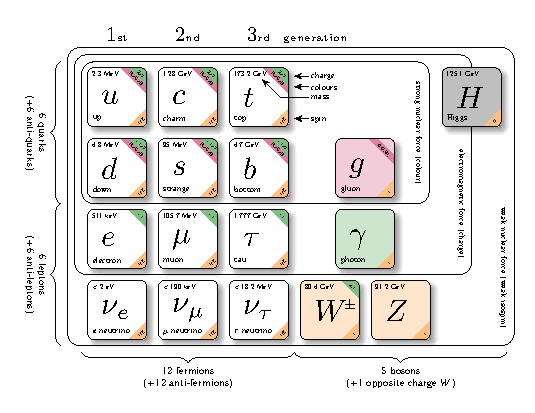
\includegraphics[width =0.85\linewidth]{Figures/Theory/standard_model.pdf}\hfill
\caption[The particle content of the SM.]{An overview of the particle content of the SM. Where relevant, particles are labelled with quantum numbers describing their spin, colour, and charge, along with their measured mass. Fermions are grouped according to their interactions through the weak, strong, and EM forces. Figure taken from Ref~\cite{shane_thesis}.}
\label{fig:the_sm}
\end{figure}

\section{Gauge fields and symmetries}

The SM is a gauge field theory, described using the Lagrangian formalism. The dynamics of such a theory can be derived from the corresponding Lagrangian using the Euler-Lagrange equations, similarly to the treatment for a classical system. The Lagrangian is typically constructed to obey an underlying symmetry of the physical system being described. According to Noether's theorem~\cite{Nother}, for every such symmetry of the Lagrangian, there exists a corresponding conserved quantity. For example, invariance of the Lagrangian under a spatial translation implies the conservation of momentum. In gauge theory, the Lagrangian is required to be invariant under \textit{local gauge transformations}, which apply a space-time dependent shift to the (unobservable) phase of the fields being described. The following sections describe the local gauge symmetries of the SM Lagrangian, and how they give rise to the fundamental forces.

\subsection{Electromagnetic interactions}

The QFT for electromagnetism is quantum electrodynamics (QED), describing charged fermions and their interactions with the photon. Terms in the corresponding QED Lagrangian that describe the spin-${\frac{1}{2}}$ fermion fields, can be grouped into the so-called Dirac Lagrangian, ${\mathcal{L}}$. This Lagrangian will be used to illustrate how imposing local gauge invariance leads naturally to the introduction of additional gauge fields. 

The Dirac Lagrangian~\cite{Thomson} has the form

\begin{equation}
    \mathcal{L} = i\bar{\psi}\gamma^{\mu}\partial_{\mu}\psi - m\bar{\psi}\psi,
\end{equation}

\noindent where ${\psi}$ is the Dirac spinor, and ${\bar{\psi}}$ is the adjoint spinor defined as ${\bar{\psi}=\psi^{\dagger}\gamma^{0}}$. The terms ${\gamma^{\mu}}$ are the ${\gamma}$-matrices which obey the anticommutation relation ${\{\gamma^{\mu},\gamma^{\nu}\} = 2\eta^{\mu\nu}}$, where ${\eta^{\mu\nu}}$ is the Minkowski metric, and ${\mu,\nu \in \{0,1,2,3\}}$. Finally, ${m}$ is the mass of the fermion described by ${\psi}$.

The Dirac Langrangian is clearly invariant under a \textit{global} gauge transformation to the fermion fields. This transformation belongs to the U(1) symmetry group, and thus can be described by a single real parameter, ${\theta}$, as

\begin{equation}
    \psi \rightarrow e^{ig\theta}\psi,
\end{equation}

\noindent where ${\theta}$ and ${g}$ are constant, real numbers. Now consider elevating this symmetry to a \emph{local} gauge transformation, of the kind
%g is obviously different for each particle though! For leptons is +/1, for quarks it is fractional

\begin{equation}
    \psi \rightarrow e^{ig\theta(x)}\psi,
\end{equation}

\noindent where ${\theta(x)}$ can now be different at any point in space-time, ${x}$. Unlike for global transformations, where the four-derivative commuted with the position independent value of ${\theta}$, the corresponding Lagrangian is no longer invariant, acquiring the additional term
%these charged g are eigenvalues of the generators.

\begin{equation}
\label{eqn:theory_LGT_1}
    \mathcal{L} \rightarrow \mathcal{L} - g\bar{\psi}\gamma^{\mu}(\partial_{\mu}\theta(x))\psi.
\end{equation}

%The dirac LAGrangian is similat to the dirac EQN, except for it has a psi(bar) to make it LGI under U(1). So in the dirac EQN, you just read off allowed vertices factors, but in the lagrangian, you read off interactions processed

\noindent To remove the residual term and restore gauge invariance, the derivative ${\partial_\mu}$ is replaced by the covariant derivative, ${D_{\mu}}$, defined as:

\begin{equation}
    D_{\mu} \equiv \partial_{\mu} + igA_{\mu},
\end{equation}

\noindent where ${A_\mu}$ is an additional field that has been added to the Dirac Lagrangian. The desired cancellation of the ${g\bar{\psi}\gamma^{\mu}(\partial_{\mu}\theta(x))\psi}$ term in Eqn~\ref{eqn:theory_LGT_1} is achieved, provided the new field transforms as

\begin{equation}
    A_{\mu} \rightarrow A_{\mu} - \partial_{\mu}\theta(x),
\end{equation}

%A_mu is g_{munu}/p^2-m^2 as seen in the usual ME. If the photon isn't intermediate, the polarisation vectors must be included
\noindent exhibiting the same gauge invariance observed in classical electromagnetism. In QED, the new boson is associated with the photon propagator, with ${g}$ then assuming the electron charge. The modified Dirac Lagrangian, which no longer describes free particle fields, and is now locally gauge invariant, can be written as:

\begin{equation}
    \mathcal{L} = i\bar{\psi}\gamma^{\mu}D_{\mu}\psi - m\bar{\psi}\psi - \frac{1}{4}F^{\mu\nu}F_{\mu\nu},
\end{equation}

\noindent where ${F^{\mu\nu}}$ is the electromagnetic field strength tensor, which is also invariant under local gauge transformations. %field tensor part gives Maxwell equations when applying equations of motions

Compared with the original Lagrangian, the term ${-g\bar{\psi}\gamma^{\mu}A_\mu\psi}$ has been added, corresponding to the basic QED interaction vertex between the fermion and photon fields, shown by the Feynman diagram in Figure~\ref{fig:theory_qed_vertex}. The photon and its interactions thus arise naturally from requiring a locally gauge invariant description of fermionic interactions. Note that mass terms for the new field, which would take the form ${-\frac{1}{2}m_{A}^{2}A_{\mu}A^{\mu}}$, are not included, since the term transforms as 

\begin{equation}
    \frac{1}{2}m_{A}^{2}A_{\mu}A^{\mu} \rightarrow \frac{1}{2}m_{A}^{2}\left(A_{\mu} - \partial_{\mu}\theta(x)\right)\left(A^{\mu} - \partial^{\mu}\theta(x)\right) \neq \frac{1}{2}m_{A}^{2}A_{\mu}A^{\mu},
\end{equation}

\noindent breaking the gauge symmetry for values of ${m_{A}\neq 0}$. This feature will become important when discussing electroweak symmetry breaking, and the non-zero weak gauge boson masses. 

\begin{figure}[htb]
  \centering
    \begin{tikzpicture}
        \begin{feynman}
        \vertex (v1) at (1,-1.5) {\(A_{\mu}\)};
        \vertex (v2) at (1.5,-1.5);
        \vertex (vg) at (3.9,-1.5) {\(g\)};
        \vertex (v3) at (3.5,-1.5);
        \vertex (v4) at (5,0) {\(\psi\)};
        \vertex (v5) at (5,-3) {\(\bar{\psi}\)};
  
 
    \diagram* {
    (v2) -- [boson] (v3),
    (v3) -- [fermion] (v4),
    (v3) -- [anti fermion] (v5),

    };
  \end{feynman}
  \end{tikzpicture}
  \caption[The fundamental QED interaction vertex.]{The fundamental QED vertex, where the photon field, ${A_{\mu}}$, interacts with a charged fermion field described by ${\psi}$.}
  \label{fig:theory_qed_vertex}
\end{figure}


\subsection{Strong interactions}

The theory of strong interactions is known as quantum chromodynamics (QCD), describing quarks, gluons, and their interaction. The corresponding Lagrangian is again formed by requiring a physical symmetry to be respected; for QCD, this symmetry is invariance under a local SU(3) gauge transformation, which has form

\begin{equation}
    \psi \rightarrow e^{ig_{s}\theta(x)^{a}\frac{\lambda^{a}}{2}}\psi,
\end{equation} %remember this is acting on a 3 component wavefunction

\noindent where ${\lambda^{a}}$ are the eight generators of the SU(3) group (${a\in\{1,2,...,8\}}$), represented by the ${3\times3}$ the Gell-Mann matrices, and ${\theta(x)^{a}}$ are eight functions of the spacetime co-ordinate, ${x}$~\cite{Thomson}. The SU(3) symmetry of the QCD interaction implies a conserved quantity, which in the case of quark and gluon fields, is the colour charge. Particles (anti-particles) with colour charge exist in one of three states, labelled red (anti-red), blue (anti-blue), and green (anti-green). %The particle wavefunctions therefore have three degrees of freedom, with one colour per degree (same maths as the uds approxmate flavour symmetry). In other words, colour is just a label for orthogonal states in colour space. %N.B. no analytical proof for colour confinement, but Lund string model is one example theory. Evidence for color: ee->qq / ee->mu mu

In order to maintain invariance, the four-derivative is modified to the covariant derivative,

\begin{equation}
    D_{\mu} \equiv \partial_{\mu} + ig_{s}\frac{\lambda^{a}}{2}G^{a}_{\mu}.
\end{equation}

\noindent This necessitates the introduction of eight new fields, ${G_{\mu}^{a}}$, which correspond to massless gluons, the mediators of the strong interaction. The value of ${g_{s}}$, therefore, is the strong force coupling strength. 

The QCD lagragian remains invariant, provided the new fields transform as

\begin{equation}
    G_{\mu}^{c} \rightarrow G_{\mu}^{c} - \partial_{\mu}\theta^{c}(x) - g_{s}f^{abc}\theta^{a}(x)G_{\mu}^{b},
\end{equation}

\noindent where ${f^{abc}}$ are the completely antisymmetric structure constants, defined by ${\left[ \lambda^{a},\lambda^{b} \right] = if^{abc}\lambda^{c}}$, which arise due to the non-abelian nature of the SU(3) group. Unlike in the case of QED, a non-abelian gauge theory permits self-interaction of the accompanying gauge bosons. This can be revealed by the required form of the field strength tensor, which for QCD is

\begin{equation}
      F^{a}_{\mu\nu} = \partial_{\mu}G_{\nu}^{a} - \partial_{\nu}G_{\mu}^{a} - g_{s}f^{abc}G^{b}_{\mu}G^{c}_{\mu}, 
\end{equation}

%this can be deriving y noting that F_{mu,nu} = (1/ig) [D^mu, D_nu]
\noindent resulting in trilinear and quartic terms in the QCD Lagrangian. Collection of the previous results together yields the final Lagrangian,

\begin{equation}
    \mathcal{L_{\mathrm{QCD}}} = \sum_{f} i\bar{\psi}_{f}(\gamma^{\mu}D_{\mu} - m_{f})\psi_{f} - \frac{1}{4}F^{a\mu\nu}F_{\mu\nu}^{a},
\end{equation}

\noindent where ${f}$ indexes the six quark flavours, with corresponding mass ${m_{f}}$. %psi here are like a 3 vector (color) of 4-vector spinors (page 246 Thompson)

An additional difference between QED and QCD is the relationship between the strength of the QCD interaction, and the interaction energy scale. The strong force interaction strength becomes larger at smaller momentum transfers, a property which results in the confinement of low energy quarks to colourless baryons and mesons. Conversely, at large energies such as those probed at the Large Hadron Collider, quarks and gluons behave as quasi-free particles, in an effect known as \textit{asymptotic freedom}.




\subsection{Electroweak unification}
%all this is saying is that the physical weak bosons and photon arise from four separate fields W1->3 + Amu, which results from the SU(2) x U(1) symmetry. The charged W boson are formed from W1 and W2, whereas the photon and Z are from combinations of W3 (Z) and Amu.

The unification of the EM and weak forces, originally conceived by Glashow, Weinberg and Salam (GWS)~\cite{Glashow,Weinberg,Salam}, consolidated the SM into its highly successful modern form. At a glance, the two forces already appear intimately linked; the coupling strengths are similar, and two of the weak bosons possess the charge of the EM interaction. The GWS model formalises these ideas into the modern gauge invariant theory.
%couplings are similar but the mass of the weak boson makes the weak force weak (Thompson Section 11.5.1)

It is useful to firstly consider the weak interaction alone, which is invariant under SU(2) transformations of the form

\begin{equation}
    \psi \rightarrow e^{ig\theta(x)^{i}\frac{\sigma^{i}}{2}}\psi,
\end{equation}

\noindent where the generators of the group have been identified as the three Pauli matrices, ${\sigma^{i}}$, and ${g}$ is the corresponding charge known as \textit{weak isospin}. Similarly to the previously discussed gauge groups, in order to respect the SU(2) symmetry, the four-derivative must be modified to its covariant form

\begin{equation}
    D_\mu \equiv \partial_\mu + ig\frac{\sigma^{i}}{2}W_{\mu}^{i},
\end{equation}
%In the DH^{dagger}DH terms later on, the form of this derviative gives rise to terms like Const(W1^2+W2^2) where it is clear that physical field with mass M=const is the combination of W1 and W1. Hence the later definitions of W+- = (W1^2+/-iW2^2), and similar for the Photon and Z fields.

\noindent which has resulted in the introduction of three new fields, ${W_{\mu}^{i}}$. Given that the group generators are 2${\times}$2 matrices, the particle states that interact through the weak force should be represented by two component vectors, which are termed \textit{weak isospin doublets}. 
%called isospin because the original isospin formulation uses an approximate SU(2) summetry

Unlike the EM and strong forces, the weak interaction does not conserve parity~\cite{ParityViolation}, meaning it is not invariant under inversion of the spatial co-ordinates. The weak interaction structure has a vector minus axial-vector form %experimental observation - other billinear covariants offer the same thing. Helicity suprressed pion decay and Wu (beta decay) give evidence for parity violation, although exact interaction structure is determined through other exps

\begin{equation}
    i\frac{g}{2\sqrt{2}} \gamma^{\mu}(1-\gamma^{5})  = i\frac{g}{\sqrt{2}} \gamma^{\mu}P_{L},
\end{equation}

\noindent where ${\gamma^{5}=i\gamma^{0}\gamma^{1}\gamma^{2}\gamma^{3}}$, and ${P_{L}}$ has been identified as the left handed chiral projection operator. Given that the action of ${P_{L}}$ on right handed particle spinors produces zero, an immediate consequence of parity violation is that only left (right) handed chiral particle (anti-particle) states may participate in weak interactions. To achieve this, only left handed particle and right handed anti-particle states are placed in weak isospin doublets, while right handed particle and left handed anti-particle states become isospin singlets, unaffected by SU(2) transformations. For this reason, the SU(2) symmetry group of the weak interactions is often referred to as SU(2)${_{\mathrm{L}}}$. %i.e. acting on singlet will return zero, acting on doublet is a rotation in SU(2) space - similar to baryon and meson approximate symmetries. Note that each particle in the doublet either a combination of weak eigenstate - for neutrinos, this mean we use the PMNS matrix, for quarks its the CKM.
%in the relativistic limit, this chirality = helicity which has consequences for allowed spin alignments (Thompson page 294). Note that neutrino spinors have a PMNS factor accounting for the flavour eignestates being a lienar combination of the mass eigenstates. Weak interaction also violates charge conjugation as it also gives RH particles. So, its plausible that CP together could be conserved, even though in reality it isn't. The non-real elements break time reversal symmetry sp, CP must be violated to keep CPT invariant. %also weird that in the WI, both quarks and neutrinos have flavour mixing matrices respectively, but leptons do not. CP violation in quark sector is seen in neutral meson mixing, in preference for particle over anti particles

In its current form, the weak interaction gauge group has three associated gauge bosons, all of which violate parity. This is, however, in contradiction with experiment, where the ${\mathrm{Z}}$ boson associated with weak neutral current interactions couples to both left handed and right handed chiral particles. The GWS model provides the resolution, where the two neutral bosons of the theory are postulated to arise from combinations of fields generated by an SU(2)${_{\mathrm{L}}\times}$U(1) symmetry. To maintain invariance under such a transformation, the covariant derivative associated with the weak interaction is updated with an additional term corresponding to the U(1) symmetry, such that overall

\begin{equation}
\label{eqn:ew_covariant_derivative}
    D_\mu \equiv \partial_\mu + ig\frac{\sigma^{i}}{2}W_{\mu}^{i} + ig'YB_{\mu},
\end{equation}

\noindent where ${Y}$ is known as the \textit{weak hypercharge}, and ${g'}$ is the associated coupling. In the GWS model, the charged weak bosons are given by combinations of the ${W^{1}_{\mu}}$ and ${W^{2}_{\mu}}$ fields,
%I again is the identity! Note that in gauage transforms to the field, g can be +1e or 2/3 etc. for charged leptons and quarks respectively; it is not fixed! Hence why Y can take different values (of charge) too.

\begin{equation}
     W^{\pm}_\mu = \frac{1}{\sqrt{2}}(W_\mu^1 \mp iW_\mu^2).
\end{equation}

\noindent The physical neutral fields of the theory, the ${\mathrm{Z}}$ boson (${Z_{\mu}}$) and the photon, are then expressed as linear combinations of the remaining ${W^{3}_{\mu}}$ boson, and the new ${B_\mu}$ field. This can be expressed succinctly as
%we know W3 is neutral because it results vertex terms coupling neutral particles (Thompson, page 417-418).

\begin{equation}
\label{eqn:Z_photon_rotation_matrix}
\begin{split}
    \begin{pmatrix}
    Z_\mu \\
    A_\mu
    \end{pmatrix} 
    &= 
    \begin{pmatrix}
    \cos{\theta_W} & -\sin{\theta_W} \\
    \sin{\theta_W} & \cos{\theta_W}
    \end{pmatrix} 
    \begin{pmatrix}
    W^3_\mu \\
    B_\mu
    \end{pmatrix}
\end{split}
,
\end{equation}

\noindent where ${\theta_{W}}$ is called the Weinberg angle, which controls the mixing. The charges associated with each transformation can be identified by considering the electroweak Lagrangian, using the definition of the covariant derivative in Eqn \ref{eqn:ew_covariant_derivative}. Terms involving right handed fields, ${\psi_{\mathrm{R}}}$, include
%sin(thetaW)^2 = 0.222

\begin{equation}
    \mathcal{L} \supset -\bar{\psi}_{\mathrm{R}}g'\cos{\theta_{W}}Y\gamma^{\mu}A_{\mu}\psi_{\mathrm{R}}.
\end{equation}


\noindent By comparison with the analogous term in the QED lagrangian, 
the relationship between ${g'\cos{\theta_{W}}=|e|}$ can be inferred, and the weak hypercharge, ${Y}$, is identified as the electric charge of the particle. Similarly, action of the covariant derivative on left handed fields, $\psi_{\mathrm{L}}$, yields terms such as,
%theta = tan(g'/g). For this part, the GFT notes and equations 6.41-6.45 clear it up, bearing in mind that the \supsets are important in understanding which terms are written explicitly. Its basically expanding the Dmu terms are subbing in for Bmu using the definitions from the rotation matrix

\begin{equation}
    \mathcal{L} \supset -\bar{\psi_{\mathrm{L}}}(g\sin{\theta_{W}}\frac{\sigma^{3}}{2} + g'\cos{\theta_{W}}Y)\gamma^{\mu}A_{\mu}\psi_{\mathrm{L}}.
\end{equation}

\noindent In order to assert that the two states in each weak doublet differ by a factor of $|e|$, the relation $g\sin{\theta_{W}}=|e|$ must hold. Finally, the observation that EM interactions do not depend on the handed-ness of the fermion, yields the relation between the generators of the neutral fields

\begin{equation}
    Q = \sigma^{3} + \frac{Y}{2}\mathbb{1}_{2}.
\end{equation}

\noindent The unification has thus allowed for a photon interaction that is invariant under a parity transformation, and the weak current interaction which is not.
%this last bit can be seen from Eq 2.22 of Jon's thesis where subbing in two terms gives the required QED vertex format.
%setting the multipliers of the fermion fields equal in 2.22 line 2 of Jon's thesis. Acting on the spinors yield his 1D equation

Whilst requiring local gauge invariance provides an elegant method to introduce interactions, as well as unify the weak and EM forces, it is, at this point, unable to permit masses for the weak gauge bosons. This prediction is in clear contradiction with the experimental observation of the massive $\mathrm{W}$ and $\mathrm{Z}$ gauge bosons. To resolve this contradiction, the BEH mechanism is introduced.

\section{Spontaneous symmetry breaking}
%breaking the SU(2) x U(1) symmetry means that below the EW scale, with no Higgs boson, only the massless field (QCD and QED) interactions occur. Above this, the weak interactions are possible, and the bosons are allowed to have mass via the Higgs which may now be produced.

In the BEH mechanism, masses of the fundamental particles are generated through spontaneous breaking of a Lagrangian symmetry. In the SM, the BEH mechanism is realised by introduction of a complex scalar doublet, with a non-zero expectation value in the vacuum state. As a result of the new field, although the Lagrangian still respects the SU(2)$_{\mathrm{L}}\times$ U(1) symmetry associated with the weak and EM gauge groups, the ground state does~\cite{BroutEnglert,HiggsBS1,HiggsBS2,HiggsBS3,Kibble}.


\subsection{Symmetry breaking for a complex scalar field}

To introduce the BEH mechanism, it is instructive to first consider the simpler case of U(1) symmetry breaking, generated by the introduction of a complex scalar field, $\phi=\frac{1}{\sqrt{2}}(\phi_{1} + i\phi_{2})$. Similarly to the QED formalism, the U(1) symmetry requires the covariant derivative to be introduced, defined as~\cite{Thomson}

\begin{equation}
    D_{\mu} \equiv \partial_{\mu} + igB_{\mu},
\end{equation}

\noindent where $B_{\mu}$ is a new massless field with its own transformation properties. The Lagrangian describing the complex scalar field therefore has the form~\cite{Thomson}

\begin{align}
\label{eqn:complex_scalar_lagrangian}
    \mathcal{L} &= (D_{\mu}\phi)^{*}(D^{\mu}\phi) -\frac{1}{4}F^{\mu\nu}F_{\mu\nu} - V(\phi) \nonumber \\
    &= (D_{\mu}\phi)^{*}(D^{\mu}\phi) -\frac{1}{4}F^{\mu\nu}F_{\mu\nu} - \mu^{2}(\phi^{*}\phi) - \lambda(\phi^{*}\phi)^{2},
\end{align}

\noindent where $V(\phi)$ is the potential energy of the field which is chosen to have form $V(\phi) =  \mu^{2}(\phi^{*}\phi) + \lambda(\phi^{*}\phi)^{2}$. For the potential to have a finite minimum, the value of $\lambda$ is constrained to positive values; however, the value of $\mu^{2}$, is not. If $\mu^{2}$ is chosen to be positive, the resulting potential has a singe minimum at $\phi=(\phi_{1},\phi_{2})=(0,0)$, representing a scalar particle with mass $\mu$. However, if the value of $\mu^{2}$ is chosen to be negative, the associated term can no longer be interpreted as a particle mass, and the potential possesses a ring of minima satisfying $\phi^{*}\phi = \phi_{1}^{2} + \phi_{2}^{2} = -\mu^{2}/\lambda = v^{2}$. The expectation value of the Higgs potential in the vacuum state is defined as $v$, indicated by the dashed line of minima in Figure~\ref{fig:higgs_potential}. Since the minima of the potential do not occur at $\phi=0$ in the case of $\mu^{2}<0$, the field is said to have a \textit{non-zero vacuum expectation value}. It is the actual choice of minimum for the vacuum state that spontaneously breaks the local gauge symmetry of the Lagrangian. Without loss of generality, the vacuum state can be chosen to lie entirely on the real axis, such that $\phi=(v,0)$. The field can then be represented as a expansion around the vacuum state

\begin{equation}
    \phi = \frac{1}{\sqrt{2}}(v + \eta + i\xi),
\end{equation}

\noindent which when substituted into the Lagrangian of Eqn \ref{eqn:complex_scalar_lagrangian}, yields terms~\cite{Thomson}

\begin{equation}
    \mathcal{L} \supset \frac{1}{2}(\partial_{\mu}\eta)(\partial^{\mu}\eta) - \lambda v^{2}\eta^{2} + \frac{1}{2}(\partial_{\mu}\xi)(\partial^{\mu}\xi) + \frac{1}{2}g^{2}v^{2}B_{\mu}B^{\mu} - \frac{1}{4}F^{\mu\nu}F_{\mu\nu}.
\end{equation}

\noindent The Lagrangian describes a massive scalar field, $\eta$, and massless boson $\xi$, which is termed the \textit{Goldstone} boson. In addition, the previously massless field $B_{\mu}$ associated with the local U(1) gauge symmetry has now acquired a mass term. The BEH mechanism therefore appears a viable method to introduce the massess of the SM vector bosons. However, the Lagrangian also contains terms such as $gvB_{\mu}\partial^{\mu}\xi$ which would appear to represent a direct coupling between the spin-0 Goldstone boson and spin-1 gauge field. In order to eliminate the Goldstone field from the Lagrangian, the \textit{unitary gauge} is adopted. This corresponds to fixing the phase of the U(1) transformation such that the scalar field can be expressed as:
% derivation in page 477 Thompson, uses taylor expansion of field. The DOF associated with the Xi field is now a longitudinal polarisation of the now massive field B.

\begin{equation}
    \phi(x) = \frac{1}{\sqrt{2}}(v+\eta) \equiv \frac{1}{\sqrt{2}}(v+h),
\end{equation}

\noindent where the field $\eta$ has been written using $h$ to emphasise that this is the physical field of the theory. Finally, ignoring constants, Eqn~\ref{eqn:complex_scalar_lagrangian} can be written as~\cite{Thomson}
\begin{equation}
\label{eqn:complex_scalar_lagrangian_full}
\begin{split}
    \mathcal{L} &= \frac{1}{2}(\partial_{\mu}h)(\partial^{\mu}h) - \lambda v^{2}h^{2} +         \frac{1}{2}g^{2}v^{2}B_{\mu}B^{\mu} - \frac{1}{4}F^{\mu\nu}F_{\mu\nu} \\
     &+ g^{2}vB_{\mu}B^{\mu}h + \frac{1}{2}g^{2}B_{\mu}B^{\mu}h^{2} - 
    \lambda vh^{3} - \frac{1}{4}\lambda h^{4}.
\end{split}
\end{equation}

\noindent The Lagrangian now describes a massive gauge boson associated with the $B_{\mu}$ field of the U(1) symmetry, and a massive scalar field, $h$, known as the Higgs field. The mass of the gauge boson can be identified as $m_{B} = gv$, while the Higgs boson mass is given by $m_{h}\equiv m_{H}=\sqrt{2\lambda}v$. The Lagrangian also contains interaction terms between the two fields, as well as triple and quartic self-interactions of the Higgs boson. The spontaneous breaking  of a U(1) local gauge invariance has therefore allowed for a previously massless field to obtain mass through introduction of a scalar field, the quanta of which is a massive boson.
%VEV = 246 GeV in the SM 

\begin{figure}[htbp!]
\centering
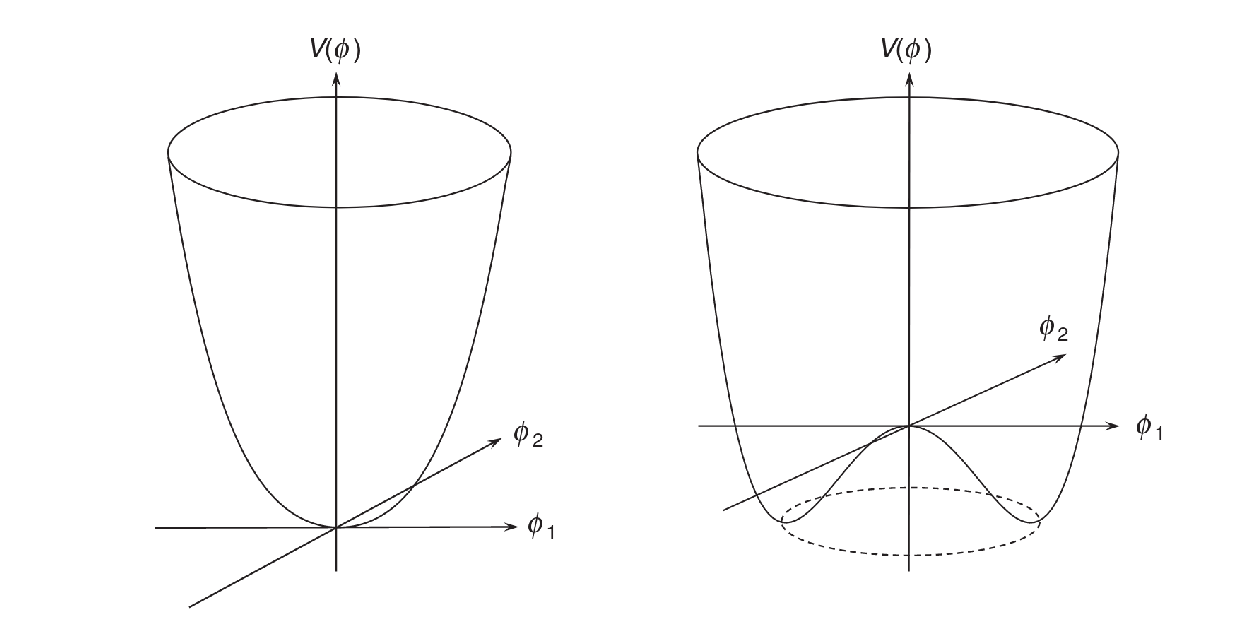
\includegraphics[width =0.7\linewidth]{Figures/Theory/higgs_potential.pdf}%
\caption[The potential for a complex scalar field.]{The potential $V(\phi) = \mu^{2}(\phi^{*}\phi) + \lambda(\phi^{*}\phi)^{2}$ for a complex scalar field. Two cases are considered: $\mu^{2}>0$ (left), where a single minima is present, and $\mu^{2}<0$ (right), where the field acquires a non-zero vacuum expectation value, with minima at $|\phi| = -\mu^{2}/\lambda = v^{2}$. Figure taken from Ref~\cite{Thomson}.}
\label{fig:higgs_potential}                                              
\end{figure}

\subsection{The SM Higgs boson}

In the SM, the Higgs field consists of two complex scalar fields, which transform as a doublet under SU(2)$_{\mathrm{L}}$ transformations. The field has four degrees of freedom, and can be written as

\begin{equation}
\begin{split}
    H =
    \begin{pmatrix}
    \phi_{+} \\
    \phi_{0}
    \end{pmatrix} 
    =  \frac{1}{\sqrt{2}} 
    \begin{pmatrix}
    \phi_{1} + i\phi_2 \\
    \phi_{3} + i\phi_4 
    \end{pmatrix} 
   \end{split},
\end{equation}

\noindent where the upper and lower components differ by one unit of charge. The corresponding Lagrangian therefore has terms

\begin{align}
\label{eqn:sm_higgs_lagrangian}
    \mathcal{L} & \supset (D_{\mu}H)^{\dagger}(D^{\mu}H) + V(H) \\
                &= (D_{\mu}H)^{\dagger}(D^{\mu}H) - \mu^{2}H^{\dagger}H - \frac{\lambda}{4}(H^{\dagger}H)^{2},
\end{align}
%the whole thing has field strength tensors too but gets messy writing it all out

\noindent where $D_\mu$ is defined for an SU(2)$_{\mathrm{L}}\times$U(1) symmetry in Eqn~\ref{eqn:ew_covariant_derivative}. The SM Higgs potential, $V(H)$, has vacuum states with non-zero expectation value that satisfy

\begin{equation}
    H^{\dagger}H = \frac{1}{2}(\phi_{1}^{2} + \phi_{2}^{2} + \phi_{3}^{2} + \phi_{4}^{2}) = -\frac{\mu^{2}}{2\lambda} = \frac{v^{2}}{2}.
\end{equation}

\noindent The vacuum state, which breaks the SU(2)$_{\mathrm{L}}\times$U(1) symmetry of the Lagrangian, is chosen to correspond to the neutral complex field. Expanding around this choice of minimum yields 

\begin{equation}
\begin{split}
    H = \frac{1}{\sqrt{2}} 
    \begin{pmatrix}
    0  \\
    v+h
    \end{pmatrix} 
   \end{split},
\end{equation}

\noindent where, again, the unitary gauge has been adopted. Inserting this into the Lagrangian of Eqn~\ref{eqn:sm_higgs_lagrangian} yields terms

\begin{align}
    \mathcal{L} &\supset \frac{1}{4}g^{2}v^{2}W^{+}_{\mu}W^{\mu -} + \frac{1}{8}(g^{2}+g^{'2})v^{2}Z_{\mu}Z^{\mu} \\
    &+ \frac{1}{2}(\partial_{\mu}h)(\partial^{\mu}h) - \lambda v^{2}h^{2},
\end{align}

\noindent where the rotation to the physical fields has been applied using Eqn~\ref{eqn:Z_photon_rotation_matrix}. The mass for the charged $\mathrm{W}$ bosons can be identified as $m_{W} = gv/2$, while the neutral $\mathrm{Z}$ (Goldstone) boson mass is $m_{Z} = v\sqrt{g^{2} + g^{'2}}/2$, both of which depend on the Higgs boson vacuum expectation value. The quanta of mass for the Higgs field can also be identified as $m_{H}=\sqrt{2\lambda}v$. No such mass terms are present for the $A_{\mu}$ field, corresponding to the photon; thus, the BEH mechanism has provided mass terms for the weak gauge bosons, while preserving the massless photon. Finally, similarly to Eqn~\ref{eqn:complex_scalar_lagrangian_full}, the Lagrangian also contains triple and quartic interaction terms between one or two Higgs bosons and the weak gauge bosons.
%with identical form/coupling strengths as seen in U(1) symmetry
%note that for a complex fied that mass term is m^2 \phi*phi but for a real field it is m^2/2 \phi^2, hence the apparent loss of a factor of two
%also note that the real photon field is not Bmu, its Amu

\subsection{Yukawa interactions}

In the SM, the BEH mechanism is also used to generate the fermion masses~\cite{Thomson}. Due to the different transformation properties of left and right handed fermions, typical mass terms of the form $-m\bar{\psi}\psi = -m(\bar{\psi}_{\mathrm{R}}\psi_{\mathrm{L}} + \bar{\psi}_{\mathrm{L}}\psi_{\mathrm{R}})$ do not respect an SU(2)$_{\mathrm{L}}\times$U(1) symmetry. However, since the Higgs field behaves as a doublet under SU(2) transformations, mass terms of the form $\bar{L}H$ respect an SU(2)$_{\mathrm{L}}$ symmetry, where $L$ represents a doublet of left handed fermions. When combined with a right handed fermion singlet, $R$, the resulting mass term $\bar{L}HR$ respects the required SU(2)$_{\mathrm{L}}\times$U(1) gauge symmetry. Hence, fermion mass terms are identified in the Lagrangian as $-g_{f}(\bar{L}HR + \bar{R}H^{\dagger}L)$, where $g_{f}$ is a coupling strength between the Higgs boson and fermion, known as the \textit{Yukawa} coupling.

To illustrate the generation of fermion massess, consider the SU(2)$_{\mathrm{L}}\times$U(1) invariant Lagrangian mass terms for the left handed doublet containing the electron, and right handed electron singlet

\begin{equation}
\label{eqn:higgs_electron_mass}
\begin{split}
    \mathcal{L} = -g_{e}
    \left[ 
    \begin{pmatrix}
    \bar{\nu}_{e} \; \bar{e}
    \end{pmatrix}    
    _{\mathrm{L}}
    \begin{pmatrix}
    \phi^{+} \\
    \phi^{0}
    \end{pmatrix} 
    e_{R} + \bar{e}_{R}
    \begin{pmatrix}
    \phi^{+*} \; \phi^{0*}
    \end{pmatrix}   
    \begin{pmatrix}
    \nu_{e} \\
    e
    \end{pmatrix} 
    _{\mathrm{L}}
    \right].
\end{split}    
\end{equation}

\noindent Inserting the SM Higgs doublet in the unitary gauge yields

\begin{equation}
    \mathrm{L} = -\frac{g_{e}}{\sqrt{2}}v(\bar{e}_{\mathrm{L}}e_{\mathrm{R}} + \bar{e}_{\mathrm{R}}e_{\mathrm{L}})   -\frac{g_{e}}{\sqrt{2}}h(\bar{e}_{\mathrm{L}}e_{\mathrm{R}} + \bar{e}_{\mathrm{R}}e_{\mathrm{L}}).
\end{equation}

\noindent The first term has the required form for fermion masses, which can be identified as $m_{e}=g_{e}v/\sqrt{2}$. Note that conversely, the Yukawa coupling to fermions is proportional to the fermion mass. The final form of Eqn~\ref{eqn:higgs_electron_mass} is therefore

\begin{equation}
    L_{e} = -m_{e}\bar{e}e - \frac{m_{e}}{v}\bar{e}eh.
\end{equation}

\noindent Alongside the mass term, the second term gives rise to a coupling between the electron and Higgs boson, as shown in the Feynman diagram of Figure~\ref{fig:h_ee_vertex}.
%note that e=eL+eR, but combinations of the same sign are killed off by parity violation

\begin{figure}[htb]
  \centering
    \begin{tikzpicture}
        \begin{feynman}
        \vertex (v1) at (1,-1.5) {\(\mathrm{H}\)};
        \vertex (v2) at (1.5,-1.5);
        \vertex (vg) at (4.2,-1.5) {\(m_{e}/v\)};
        \vertex (v3) at (3.5,-1.5);
        \vertex (v4) at (5,0) {\(e^{+}\)};
        \vertex (v5) at (5,-3) {\(e^{-}\)};
  
 
    \diagram* {
    (v2) -- [dashed] (v3),
    (v3) -- [fermion] (v4),
    (v3) -- [anti fermion] (v5),

    };
  \end{feynman}
  \end{tikzpicture}
  \caption[The interaction between the Higgs boson and electron pair.]{Interaction vertex between the Higgs boson and electron pair.}
  \label{fig:h_ee_vertex}
\end{figure}

%make sure you know how quark massess are generated using conjugate doublet (page 485 Thompson)

\section{Higgs boson phenomenology at the LHC}

With the discovery of the Higgs boson~\cite{Aad:2012tfa,Chatrchyan:2012xdj,Chatrchyan:2013lba}  by the CMS and ATLAS experiments at the LHC, focus has shifted to performing a detailed characterisation of the new particle. This includes an extensive programme of precision measurements, as well as searches for rare and exotic decay modes. At a hadron collider such as the LHC, the Higgs boson has a rich phenomenology, allowing for measurements across various combinations of production processes and decay channels. This section describes the prominent production mechanisms and decay channels used in many SM Higgs boson analyses at the LHC.

\subsection{Higgs boson production modes}

At the LHC, where protons are brought into collision at a centre-of-mass energy of \sqrts~TeV, the Higgs boson is produced through a variety of different mechanisms, the cross sections of which are given in Table~\ref{tab:higgs_prod_xs}. The most common production process at the LHC is gluon fusion, where the Higgs boson is produced via a heavy quark loop. This is followed by vector boson fusion, where the Higgs boson is produced in association with two quarks, which hadronise to form sprays of particles known  as (hadronic) jets. Production in association with a vector boson (VH), and with a pair of top (\ttH) or bottom ($\mathrm{b}\bar{\mathrm{b}}$H) quarks are the next most common modes, followed by production in association with a single top quark. Figure~\ref{fig:higgs_prod_feynmans} gives example leading order Feynman diagrams for the four Higgs boson production modes with the highest cross section at the LHC, all of which have now been observed experimentally~\cite{CMSHiggsNature,ATLAS_HComb}.

The experimental sensitivity to each production mode depends not only on the cross section, but also on the presence of competing processes known as background events. Many production modes benefit from the presence of characteristic final state objects, which can be used to more easily identify the process.  For example, VBF Higgs boson production is characterised by two forward jets with large invariant mass, while \ttH production typically results in high multiplicity final states involving B hadrons. Utilising these features results in significant suppression of background events, allowing for more sensitive measurements to be performed.

\begin{table}[htbp!]
\centering
\caption[Cross sections for Higgs boson production at \sqrts~TeV at the LHC.]{Cross sections for the leading Higgs boson production modes at \sqrts~TeV, for a nominal Higgs boson mass of \mH= 125.0~GeV. The VH mode is split into contributions involving the $\mathrm{Z}$ and $\mathrm{W}$ gauge bosons. All values are taken from Ref~\cite{YR4}.}
\label{tab:higgs_prod_xs}
\begin{tabular}{l|cccccccc}
\hline
Production mode    & \ggH  & VBF   & $\mathrm{W}\mathrm{H}$   & $\mathrm{Z}\mathrm{H}$   & \ttH & $\mathrm{b}\bar{\mathrm{b}}$H & $\mathrm{t}$H \\ \hline
Cross section (pb) & 48.58 & 3.78  & 1.37 & 0.76 & 0.51 & 0.49                          & 0.09 \\
\hline
\end{tabular}                  
\end{table}  


\begin{figure}
        \centering
        %ggH
        \begin{subfigure}[htbp!]{0.475\textwidth}   
            \centering 
            \begin{tikzpicture}[scale=0.6]
            \begin{feynman}
                \vertex (v1) at (0,0) {\(g\)};
                \vertex (v2) at (0,-4) {\(g\)};
                \vertex (v3) at (2.5,0);
                \vertex (v4) at (2.5,-4);
                \vertex (v5) at (5.5,-2);
                \vertex (v6) at (7.8,-2) {\(\mathrm{H}\)};
    
                %label rogue t's
                \vertex (v7) at (2,-2) {\(\mathrm{t}\)};
                \vertex (v8) at (4.1,-4) {\(\mathrm{t}\)};
                \vertex (v8) at (4.1,0) {\(\mathrm{t}\)};
    
                \diagram* {
                (v1) -- [gluon] (v3) -- [anti fermion] (v5) --[dashed](v6),
                (v2) -- [gluon] (v4) -- [fermion] (v5),
                (v3) -- [fermion](v4), 
                };
        \end{feynman}
        \end{tikzpicture}
        \end{subfigure}\hfill%
        %VBF
        \begin{subfigure}[htbp!]{0.475\textwidth}
            \centering
            \begin{tikzpicture}[scale=0.7]
            \begin{feynman}
                \vertex (v1) at (0,-0.5) {\(q\)};
                \vertex (v2) at (2,-0.5);
                \vertex (v3) at (2,-3.5);
                \vertex (v4) at (0,-3.5) {\(q\)};
                \vertex (v5) at (4, 0.5) {\(q'\)};
                \vertex (v6) at (4, -4.5) {\(q'\)};
                \vertex (v7) at (3,-2);
                \vertex (v8) at (5, -2){\(\mathrm{H}\)};
  
                \vertex (vW1) at (3.6,-1.1) {\(\tiny{\mathrm{Z}/\mathrm{W}^{\pm}}\)}; %vertex labelling the rogue W/Z bosons
                \vertex (vW2) at (3.6,-3) {\(\tiny{\mathrm{Z}/\mathrm{W}^{\mp}}\)}; %vertex labelling the rogue W/Z bosons
    
                 \diagram* {
                 (v1) -- [fermion] (v2),
                (v2) -- [fermion](v5),
                (v4) -- [fermion] (v3) -- [fermion](v6),
                (v3) -- [boson](v7) -- [dashed](v8),
                (v2) -- [boson](v7)
                };
                \end{feynman}
            \end{tikzpicture}
        \end{subfigure}
        \vskip\baselineskip
        %VH
        \begin{subfigure}[htbp!]{0.475\textwidth}  
            \centering 
            \begin{tikzpicture}[scale=0.9]
            \begin{feynman}
                \vertex (v0) at (0,0) {\(q\)};
                \vertex (v1) at (0,-3) {\(\overline{q}\)};
                \vertex (v2) at (1.5,-1.5);
                \vertex (v3) at (3.5,-1.5);
                \vertex (v4) at (5,0){\(\tiny{\mathrm{Z}/\mathrm{W}^{\pm}}\)};
                \vertex (v5) at (5,-3) {\(\mathrm{H}\)};
        
                \vertex (vW1) at (2.7,-1) {\(\tiny{\mathrm{Z}/\mathrm{W}^{\pm}}\)}; %vertex labelling the rogue W/Z bosons
        
 
                \diagram* {
                (v0) -- [fermion] (v2) -- [boson] (v3) --[boson](v4),
                (v1) -- [fermion] (v2),
                (v3) -- [dashed] (v5),
                 };
            \end{feynman} 
            \end{tikzpicture}
        \end{subfigure}\hfill%
        %ttH
        \begin{subfigure}[htbp!]{0.475\textwidth}   
            \centering
            \begin{tikzpicture}[scale=0.7]
            \begin{feynman}
                \vertex (v1) at (0,0) {\(g\)};
                \vertex (v2) at (0,-2) {\(g\)};
                \vertex (v3) at (2.5,0);
                \vertex (v4) at (2.5,-2);
                \vertex (v5) at (4.5,-1);
                \vertex (v6) at (6.5,-1) {\(\mathrm{H}\)};
                \vertex (v7) at (3.8,-1.8) {\(\mathrm{t}\)};
    
                \vertex (v8) at (5.5,1.1) {\(\mathrm{t}\)};
                \vertex (v9) at (5.5,-3.1) {\(\overline{\mathrm{t}}\)};
    
                \diagram* {
                (v1) -- [gluon] (v3) -- [anti fermion,edge label=\(\overline{\mathrm{t}}\)] (v5) --[dashed](v6),
                (v2) -- [gluon] (v4) -- [fermion] (v5),
                (v3) -- [fermion] (v8),
                (v4) -- [anti fermion] (v9),
            };
            \end{feynman}
            \end{tikzpicture}
        \end{subfigure}\hfill%
    \caption[Example Feynman diagrams for Higgs boson production at the LHC.]{Example Feynman diagrams for the four dominant Higgs boson production mechanisms at the LHC. On the top row are the \ggH (left) and VBF (right) processes, while the bottom row shows the VH (left) and \ttH (right) processes.}
    \label{fig:higgs_prod_feynmans}
\end{figure}

\subsection{Higgs boson decay channels}

The Higgs boson is unstable, surviving for an extremely short time before decaying to lighter particles. These decay products are used to reconstruct the properties of the original Higgs boson. Since the Higgs boson coupling strength is proportional to the mass of the coupled particle(s), decay channels involving heavy particles are favoured. Consequently, almost 60\% of all Higgs bosons decay to two $\mathrm{b}$ quarks. It might therefore be concluded that measurements in the $\mathrm{H}\rightarrow\mathrm{b}\bar{\mathrm{b}}$ channel are the most sensitive; however, at the LHC, this considerable branching fraction is offset by the large background resulting from QCD processes, which produce a signature similar to the two jets found in the $\mathrm{H}\rightarrow\mathrm{b}\bar{\mathrm{b}}$ final state. In contrast, although the branching fraction for channels such as $\mathrm{H}\rightarrow\gamma\gamma$ is comparatively small at ${\approx}0.23\%$, the two final state photons produce a particularly clean signature which is more easily resolvable against background processes. The diphoton channel, which proceeds by a heavy particle loop, was therefore observed to have the highest sensitivity of all measured decay channels at the time of the Higgs boson discovery~\cite{Aad:2012tfa,Chatrchyan:2012xdj,Chatrchyan:2013lba}, while the $\mathrm{H}\rightarrow\mathrm{b}\bar{\mathrm{b}}$ process was only observed later in Run 2 of the LHC operation~\cite{CMSHbb,ATLASHbb}. The branching fractions for a range of Higgs boson decay channels are given in Table~\ref{tab:higgs_decay_brs}, with selected Feynman diagrams shown in Figure~\ref{fig:higgs_decay_feynmans}.

Although unsuitable for precision measurements of Higgs boson properties, rarer decay channels may also be used to study the SM predictions. These decays typically involve light particles, including channels such as $\mathrm{H}\rightarrow\mu\mu$, $\mathrm{H}\rightarrow \mathrm{c}\bar{\mathrm{c}}$, and decays to the lightest charged leptons, \Hee. The branching fraction for \Hee decays predicted by the SM is extremely small, at $\BHee \approx 5.2\times10^{-9}$. Clearly, a decay channel of this rarity is inaccessible with the data collected at the LHC during Run 2 operation; however, enhancements to \BHee are predicted under several BSM scenarios. The simplest of these are models postulating additional Higgs doublets (2HDM)~\cite{BSM_vecferm,BSM_2HDM}. Models that allow for an enhancement in $\kappa_e$ are restricted to non-flavour conserving 2HDM scenarios, given current signal strength measurements in the \Hmumu and \Htautau channels~\cite{CMSHMuMu,CMSHtautau,ATLASHtautau}. Other extensions to the SM include the addition of new higher order operators to the SM Lagrangian, including dimension 10 operators that could modify the electron Yukawa coupling by a factor of ${\approx}10$~\cite{dim_ten_operators}. 

\begin{table}[htbp!]
\centering
\caption[Branching fractions for selected Higgs boson decay modes, assuming \mH= 125.0~GeV.]{Branching fractions for a selection of Higgs boson decay modes, assuming \mH= 125.0~GeV. All values are taken from Ref~\cite{YR4}.}
\label{tab:higgs_decay_brs}
\begin{tabular}{l|ccccccccc}
\hline
Decay channel          & $\mathrm{b}\bar{\mathrm{b}}$ & $\mathrm{WW}^{*}$ & $gg$ & $\tau\tau$ & $\mathrm{c}\bar{\mathrm{c}}$ & $\mathrm{Z}\mathrm{Z}^{*}$ & $\gamma\gamma$ & $\mu\mu$ & $ee$ \\ \hline
Branching fraction (\%) & 58.2                        & 21.4    & 8.2  & 6.3       & 2.9       & 2.6     & 0.23           & 0.022     & $5.2\times10^{-9}$\\                                                                              
\hline
\end{tabular}                  
\end{table}  


\begin{figure}
        \centering
        %Hll
        \begin{subfigure}[htbp!]{0.33\textwidth}
            \centering 
            \begin{tikzpicture}[scale=0.6]
            \begin{feynman}
                \vertex (v1) at (0,-2) {\(\mathrm{H}\)};
                \vertex (v2) at (2.3,-2);
                \vertex (v3) at (5,-0.2) {\(\mathrm{f}\)};  
                \vertex (v4) at (5,-3.8) {\(\bar{\mathrm{f}}\)};
            
                \diagram* {
                (v1) -- [dashed] (v2),
                (v2) -- [fermion] (v3),
                (v2) -- [anti fermion](v4), 
                };
        \end{feynman}
        \end{tikzpicture}
        \end{subfigure}\hfill
        %Hgg
        \begin{subfigure}[htbp!]{0.33\textwidth}   
            \centering 
            \begin{tikzpicture}[scale=0.6]
            \begin{feynman}
                \vertex (v1) at (8,0) {\(\gamma\)};
                \vertex (v2) at (8,-4) {\(\gamma\)};
                \vertex (v3) at (5,0);
                \vertex (v4) at (5,-4);
                \vertex (v5) at (2.3,-2);
                \vertex (v6) at (0,-2) {\(\mathrm{H}\)};
    
                %label rogue t's
                \vertex (v7) at (5.5,-2.2) {\(\mathrm{t}\)};
                \vertex (v8) at (3.8,-3.8) {\(\mathrm{t}\)};
                \vertex (v8) at (3.8,0) {\(\mathrm{t}\)};
    
                \diagram* {
                (v1) -- [gluon] (v3) -- [anti fermion] (v5) --[dashed](v6),
                (v2) -- [gluon] (v4) -- [fermion] (v5),
                (v3) -- [fermion](v4), 
                };
        \end{feynman}
        \end{tikzpicture}
        \end{subfigure}\hfill
        %HZZ
        \begin{subfigure}[htbp!]{0.33\textwidth}
            \centering 
            \begin{tikzpicture}[scale=0.6]
            \begin{feynman}
                \vertex (v1) at (0,-2) {\(\mathrm{H}\)};
                \vertex (v2) at (2.3,-2);
                \vertex (v3) at (4,-0.6);  
                \vertex (v4) at (4,-3.4);
                
                \vertex (v5) at (6.4,0.4) {\(\mathrm{f}\)};  
                \vertex (v6) at (6.4,-1.4) {\(\bar{\mathrm{f}}\)};
            
                \vertex (v7) at (6.4,-2.4) {\(\mathrm{f}\)};  
                \vertex (v8) at (6.4,-4.4) {\(\bar{\mathrm{f}}\)};
            
                %label Z's
                \vertex (v9) at (2.9,-0.7) {\(\mathrm{Z}\)};  
                \vertex (v10) at (2.9,-3.3) {\(\mathrm{Z}^{*}\)};  
            
                \diagram* {
                (v1) -- [dashed] (v2),
                (v3) -- [fermion] (v5),
                (v3) -- [anti fermion] (v6),
                (v2) -- [boson] (v3),
                (v2) -- [boson](v4),
                (v4) -- [fermion](v7),
                (v4) -- [anti fermion](v8)
                };
        \end{feynman}
        \end{tikzpicture}
        \end{subfigure}\hfill
    \caption[Example Feynman diagrams for a selection of Higgs boson decays.]{Example Feynman diagrams for three Higgs boson decay channels: decay to two fermions (left), decay to a photon pair (centre), and decay to two $\mathrm{Z}$ bosons, which subsequently decay to fermions (right). Note that when labelling all particles, it is implicit that the invariant mass of the decay products does not exceed that of the decaying particle, with the notable exception of the virtual $\mathrm{Z}^{*}$ in the $\mathrm{H}\rightarrow \mathrm{Z}\mathrm{Z}^{*}$ decay channel.}
    \label{fig:higgs_decay_feynmans}
\end{figure}

\section{Conclusion}

The standard model of particle physics describes the fundamental particles and their interactions, and has been extraordinarily successful in explaining many experimental observations. The SM is a gauge field theory, built on an underlying $\mathrm{SU(3)}\times \mathrm{SU(2)_{L}} \times \mathrm{U(1})$ symmetry of the associated Lagrangian. The formalism allows for interactions between particles to be introduced as a required consequence of this invariance, including self-interactions between the gauge bosons. The BEH mechanism provides a tool for both bosons and fermions to acquire mass, through the introduction of a complex scalar doublet with non-zero expectation value in the vacuum state. The quanta of this field, the Higgs boson, was discovered in 2012 at the Large Hadron Collider, where it is produced through a variety of production modes. Properties of the Higgs boson are inferred from its decay products, with particularly sensitive channels including \Hgg and $\mathrm{H}\rightarrow \mathrm{Z}\mathrm{Z}^{*}$ decays. This thesis describes a search for the extremely rare decay of the Higgs boson to an electron pair.

